\documentclass{jlreq}
\usepackage{graphicx}
\usepackage{amsmath,amssymb,mathtools,bm}
\usepackage{siunitx}
\sisetup{per-mode=symbol}
\usepackage{physics}
\usepackage{mhchem}
\usepackage{booktabs}
\usepackage{ascmac}
\usepackage{hyperref}
\hypersetup{colorlinks=true,linkcolor=black,urlcolor=blue,citecolor=black}
\usepackage{enumitem}
\usepackage{geometry}
\usepackage{caption}
\usepackage{makecell} % ← セル内改行・回転文字用




\title{クーロンの法則}
\author{学籍番号：2225091~~~~~~氏名 : 西亦 岳雄}

\begin{document}

\maketitle

% ===== 目的 =====

\begin{itembox}[l]{\large 実験の目的}

　2つの小球を帯電させ, その小球間に働くクーロン力が, 小球間の距離の2乗に反比例するというクーロンの法則を電気振りこを用いることで確認する. また, 小球に帯電した電気量も確かめる. 

\end{itembox}


% ===== 原理 =====
\section*{1.原理}
　一般に, 点電荷$q_1$の周りには電場ができる. そこで, 試電荷$q_2$を点電荷$q_1$の周りに距離$r$だけ離れた位置におくと, この二つの点電荷の間には$q_1, q_2$の間の距離の2乗に反比例するクーロン力が働く($q_1,q_2が同符号のときは斥力, 異符号のときは引力が働く$). 
\begin{align}
    \bm{F}(\bm{r}) = \frac{1}{4\pi \epsilon_0} \frac{q_1 q_2}{r^2} \bm{e_r}
\end{align}

\begin{align}
    F = \frac{1}{4\pi \epsilon_0} \frac{q_1 q_2}{r^2}.
\end{align}
ここで，$\epsilon_0$ は真空の誘電率で，その値は $\epsilon_0 = 8.85 \times 10^{-12}\ \mathrm{C^2/(N\,m^2)}$ である．\par

図1,2は実験装置を小球の衝突面から垂直に見たときの図である. 物理スタンドに固定した2本の支持棒から糸で吊るした2つの小球に同符号で同量の電荷$q$を与えると, 二つの小球は反発し合い, 図1のように糸の張力$S$, クーロン力$F$, 小球にかかる重力$mg$, で理想的にはつり合う(実際の実験では, 少なからず小球は揺れ動く).図2のように, 小球が運動する軌道上でのつり合いにおいて, 張力$S$は常に軌道に垂直な方向に働くのでその成分は0であることから
\begin{align}
    F \cos \theta = mg \sin \theta
\end{align}
が成り立つ. また, $\theta$が小さいときには$h \approx l$と近似できるので
\begin{align}
    \tan \theta = \frac{d}{h} \approx \frac{d}{l} = \frac{r-r_0}{2l}.
\end{align}
(3),(4)式より
\begin{align}
    F = \tan \theta・mg = \frac{r-r_0}{2l}・mg
\end{align}
となり
\begin{align}
    \frac{1}{4\pi \epsilon_0}・\frac{q_1 q_2}{r^2} = \frac{mg}{2l}・(r-r_0)
\end{align}
が成り立つ. (6)式から
\begin{align}
    \frac{1}{r^2} = \frac{2\pi \epsilon_0 mg}{l q^2}(r-r_0)
\end{align}
を得る. 




% ===== 図1図2 =====
\begin{figure}[hbtp]
  \centering

  \begin{minipage}[b]{0.48\linewidth}
    \centering
    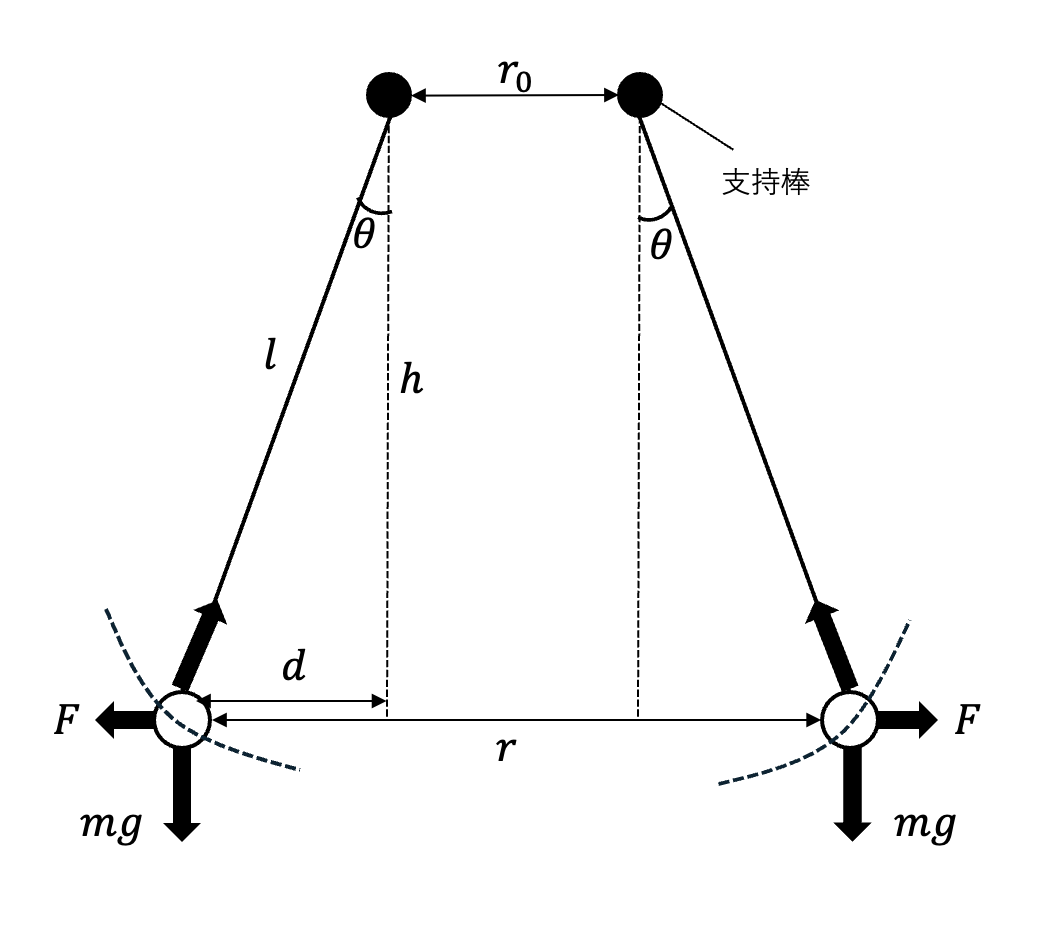
\includegraphics[width=\linewidth]{images/cou1.png}
    \caption{実験装置図1}
  \end{minipage}
  \hfill
  \begin{minipage}[b]{0.48\linewidth}
    \centering
    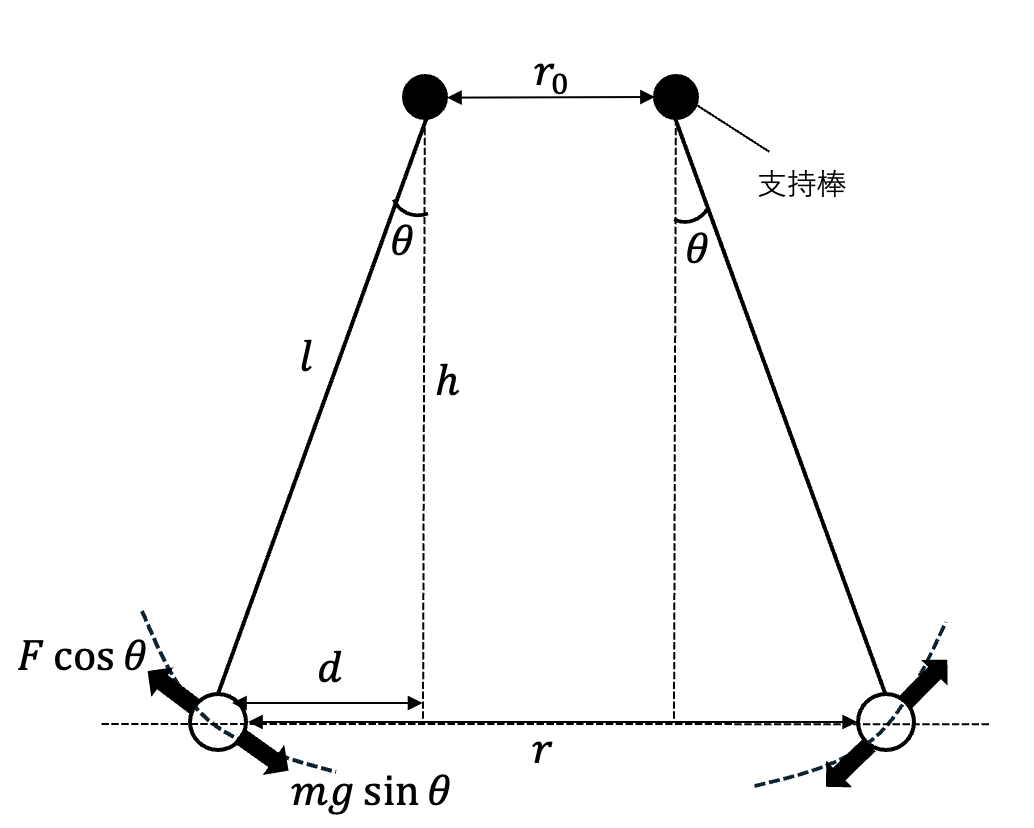
\includegraphics[width=\linewidth]{images/cou2.png}
    \caption{実験装置図2}
  \end{minipage}

\end{figure}





% ===== 実験装置構成・方法 =====
\section*{2.実験装置構成・方法}
実験装置構成と実験方法に関して述べる. 実験装置の具体的な構成は図3の通りで, 支持棒に糸を取り付け糸の先に小球を設置した. 小球間の距離はレーザーポインターを取り付けたノギスで測った.



% ===== 図3 =====
\begin{figure}[hbtp]
  \centering
  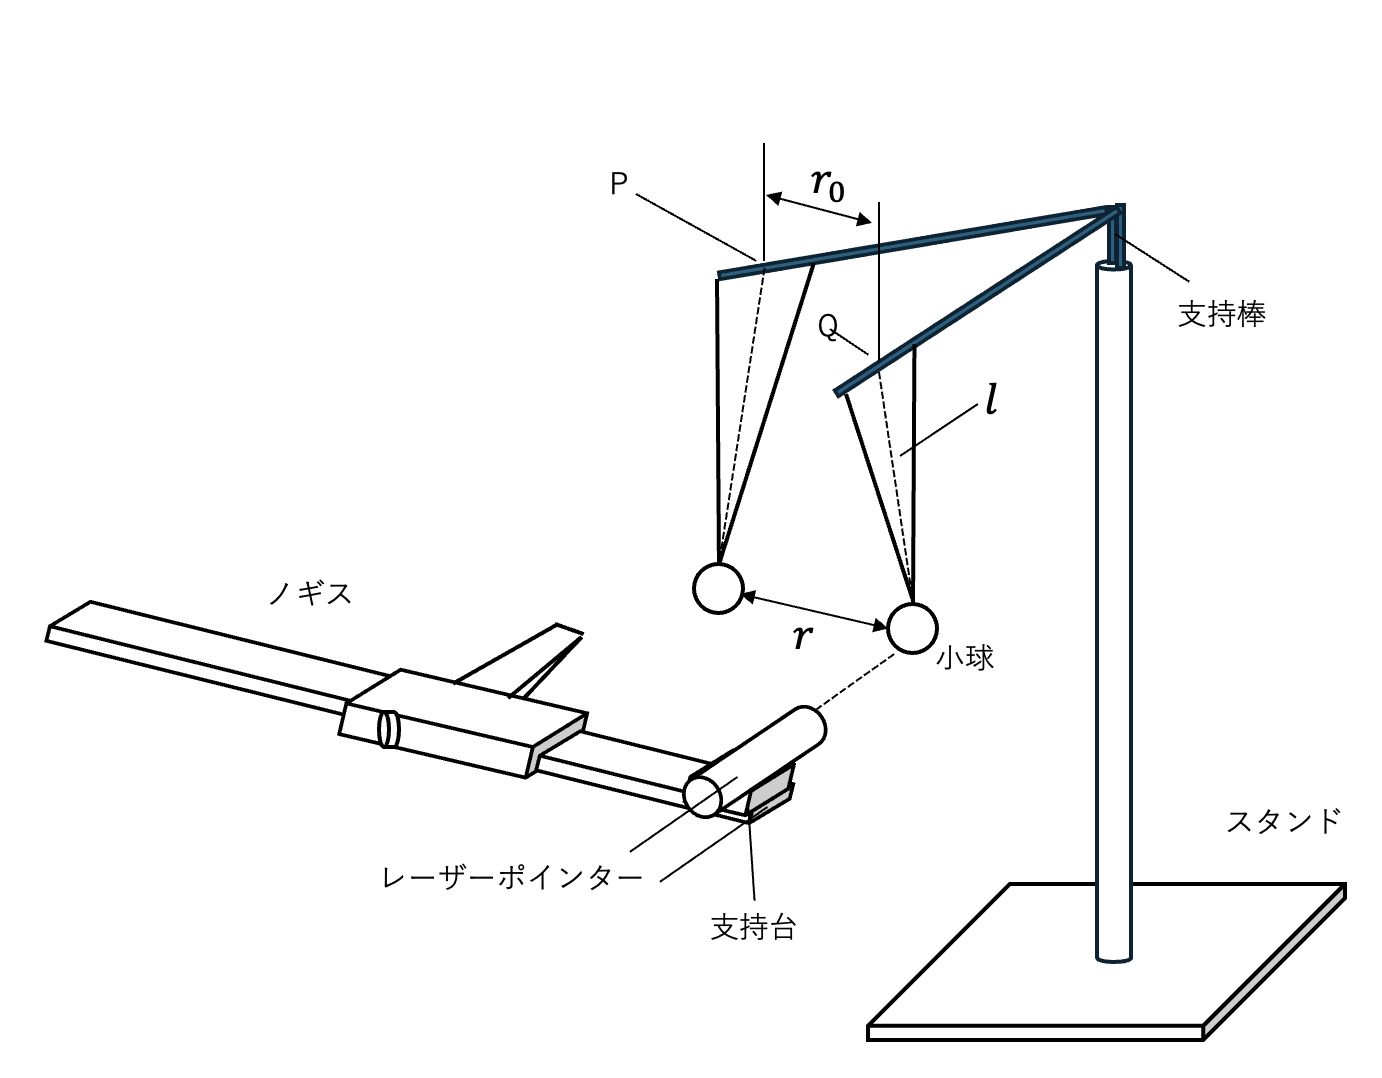
\includegraphics[width=1.0\linewidth]{images/cou3.png} % ← 拡張子・大文字小文字に注意！
  \caption{実験装置図}
\end{figure}



実際の実験方法は以下の通りである. 

①合成樹脂棒を布で擦って帯電させ, 小球をに接触させて小球に電荷を移した.\par
②図1における, P,Q間をある距離$r_0$(m)だけ離し, その距離を計測した.\par
③ノギスにレーザーポインターを固定し, 小球間の距離$r$(m)を[mm]単位の精度で計測した. 放電が進むため, 手早く計測した.\par
④$r_0$を変化させながら距離$r$の測定を繰り返し, 5点測定した.\par
⑤距離$r$の測定を終えたら, クーロンメーターで左右の小球の電荷量($q_1,q_2$)(nC)を測定した.\par


ただし, 小球の質量 $m = 0.075\,\mathrm{g}$、糸の長さ $l = 10.5\,\mathrm{cm}$、重力加速度 $g = 9.80\,\mathrm{m/s^{2}}$である.


% ===== 結果・解析 =====
\section*{3.結果・解析}
実際の測定値とそこから求められる$r-r_0$,$1/r^2$を表1にまとめた. また, 表1をグラフとしたものが図4である.



\begin{table}[htbp]
  \centering
  \caption{測定データ(小球間距離 $r$，基準距離 $r_{0}$，変位 $r-r_{0}$，および $1/r^{2}$ の計算値)}
  \label{tab:coulomb_data2}
  \begin{tabular}{|c|c|c|c|}
    \hline
    $r_{0}$ (m) & $r$ (m) & $r - r_{0}$ (m) & $1/r^{2}$ (m$^{-2}$) \\ \hline
    0.030  & 0.0476  & 0.0176  & 441.35 \\ \hline
    0.040  & 0.05425 & 0.01425 & 339.78 \\ \hline
    0.050  & 0.06050 & 0.01050 & 273.21 \\ \hline
    0.060  & 0.06810 & 0.00810 & 215.63 \\ \hline
    0.070  & 0.07300 & 0.00300 & 187.65 \\ \hline
  \end{tabular}
\end{table}


% ===== 図4 =====
\begin{figure}[hbtp]
  \centering
  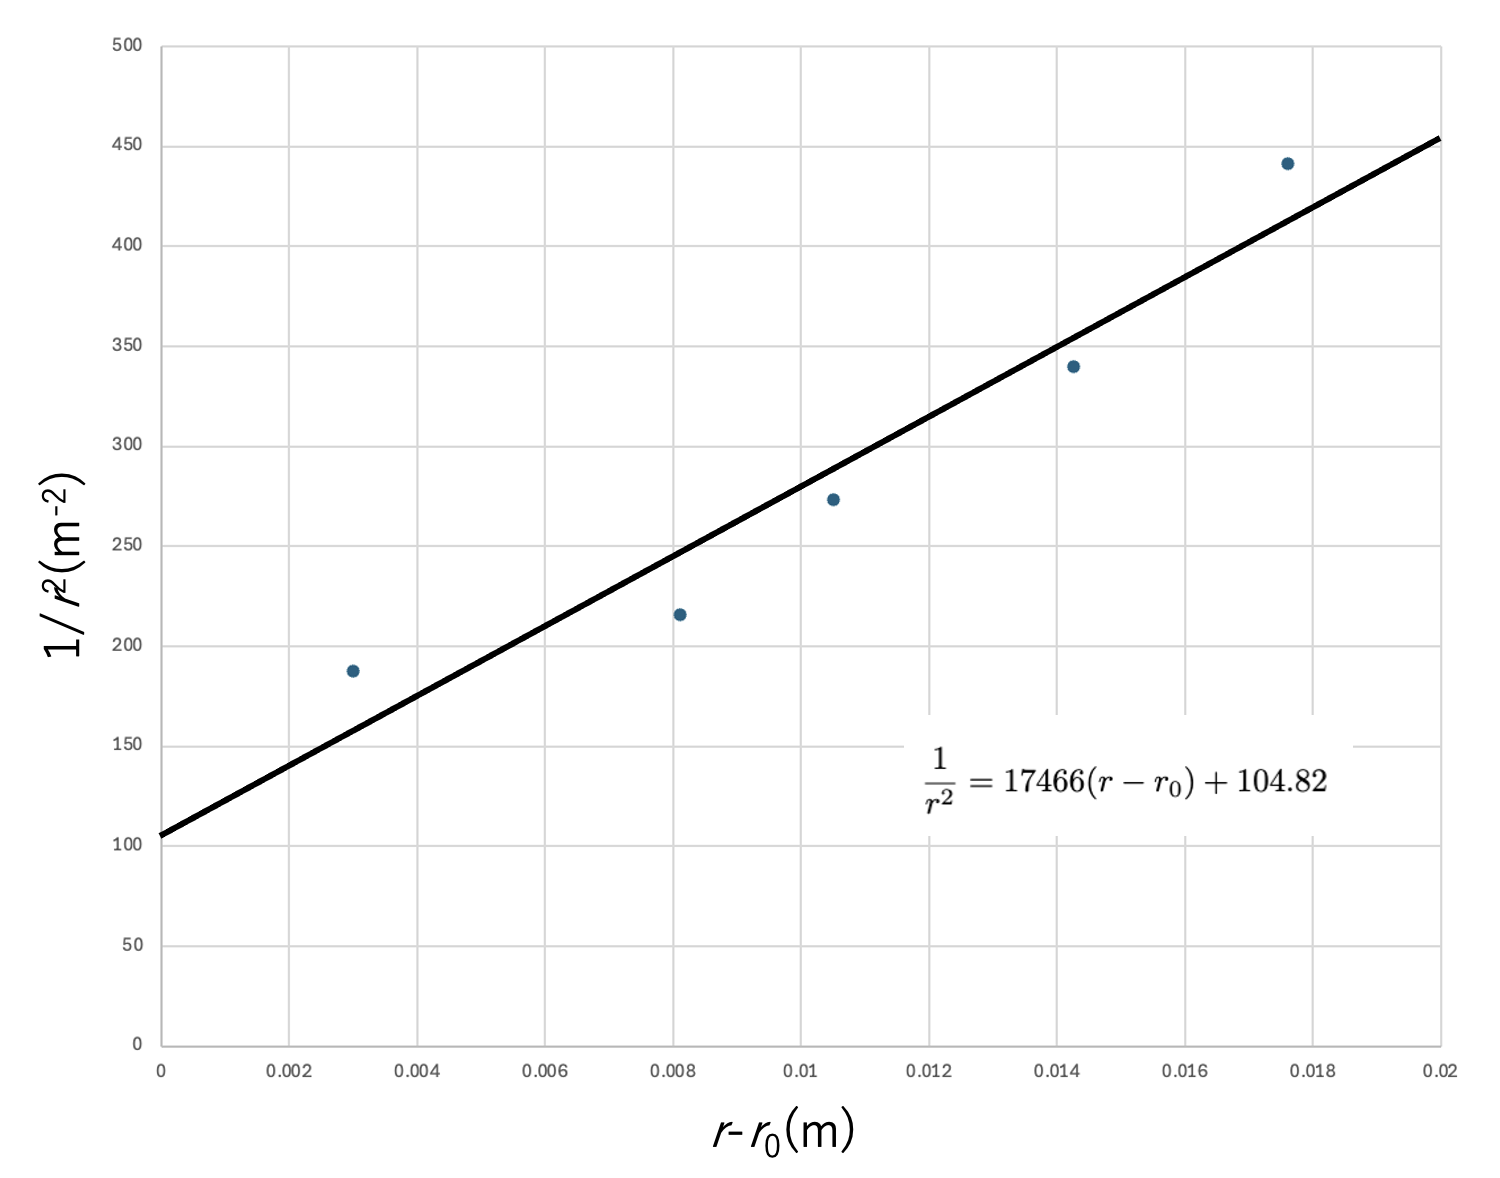
\includegraphics[width=1.0\linewidth]{images/cou4.png} % ← 拡張子・大文字小文字に注意！
  \caption{表1の測定値を用いた$r-r_{0}$ と $1/r^{2}$ のグラフ}
\end{figure}


図4から得られる関係式は(7)式より
\begin{align}
    \frac{1}{r^2} = 17466(r-r_0) + 104.82
\end{align}
である. (8),(7)式から
\begin{align}
    \frac{2\pi \epsilon_0 mg}{l q^2} = 17466
\end{align}
となり, これから電荷$q$を求めると$q \simeq 4.72 \times 10^{-9}$Cとなった. 小球に含まれる電荷をクーロンメーターで測ったその値は$q_1 = 1.4, q_2 = 5.7$であり, その平均$q_{実測値} = 3.55 \times 10^{-9}$と比べると誤差は25％でありばらつきが多いとされる今回の実験ではかなり良い結果が得られた.


% ===== 考察 =====
\section*{4.考察}
今回の実験では良い結果が得られたが, クーロンメーターで測定した電荷量とグラフの傾きから求めた電荷量とでは差がある. この点に関して考察する. \par
まず, 距離$r$における測定誤差に依存していることは確かである. 小球を帯電させた後, 小球から電荷は放電するので小球の揺れが収まる前にノギスによって計測を始めていた. $r$の計測が$\pm 0.5$mmずれるだけでも$\frac{1}{r^2}$でグラフにプロットするので傾きに大きく影響する.



% ===== 概括 =====
\section*{5.概括}


\end{document}




